%!TeX program = xelatex
% Compile with XeLaTeX or LuaLaTeX (required: the chapters contain Unicode
% math symbols -- chi-square, multiplication sign, superscript exponents --
% that pdfLaTeX will not render correctly).
% Overleaf reads the "%!TeX program" line above to auto-select the engine.
\documentclass[12pt, a4paper]{report}

\usepackage{fontspec}
\usepackage{longtable}
\usepackage{booktabs}
\usepackage{graphicx}
\usepackage[margin=1in]{geometry}
\usepackage{hyperref}

% Rename the auto-generated bibliography heading from "Bibliography"
% to "References" (BITS format).
\renewcommand{\bibname}{References}

\title{Agentic Artificial Intelligence System for Autonomous Test Script Generation and Optimization}
\author{Saif Afzal}
\date{August 2026}

\begin{document}

\begin{titlepage}
\centering
\textbf{AGENTIC ARTIFICIAL INTELLIGENCE (AI) SYSTEM FOR AUTONOMOUS TEST
SCRIPT}

\textbf{GENERATION AND OPTIMIZATION}

AIMLCZG628T: Dissertation

by

\textbf{SAIF AFZAL}

2024AA05546

Dissertation work carried out at

\textbf{3PILLAR GLOBAL, NOIDA, INDIA}

Submitted in partial fulfilment of M.Tech (Artificial Intelligence \&
Machine Learning)

degree programme

Under the Supervision of

\textbf{BILAL HASAN KHAN}

Associate Director

3Pillar Global, Noida

\IfFileExists{images/bits-logo.png}{%
  \begin{center}
\includegraphics[width=3cm]{images/bits-logo.png}\end{center}}{%
  {[}BITS Pilani institutional crest --- save the logo as
  images/bits-logo.png to replace this placeholder{]}}

\textbf{BIRLA INSTITUTE OF TECHNOLOGY \& SCIENCE}

\textbf{PILANI (RAJASTHAN)}

August 2026

\end{titlepage}

\pagenumbering{roman}
% Per the WILP guidelines (sec 1.2), Acknowledgements is the second page
% (after the title page / certificate) and the Abstract Sheet is the third.

\chapter*{Acknowledgements}
\addcontentsline{toc}{chapter}{Acknowledgements}

% Guideline order: Head of the organization -> Supervisor & Additional
% Examiner -> Professional Expert / In-charge -> Faculty mentor -> others.
% Bracketed [TO FILL] items below need real names before submission.

I express my sincere gratitude to \textbf{[TO FILL: Name, Head of the
Organization]}, 3Pillar Global, for fostering an environment supportive
of applied research alongside professional responsibilities.

I am deeply grateful to my supervisor, Mr.~Bilal Hasan Khan, Associate
Director at 3Pillar Global, Noida, for his consistent guidance,
technical scrutiny, and constructive feedback throughout every phase of
this dissertation, from the initial dataset design through to the final
statistical evaluation. His willingness to engage closely with both the
research questions and the practical engineering challenges encountered
along the way materially shaped the quality of this work. I also thank
my additional examiner, \textbf{[TO FILL: Name, Designation ---
Additional Examiner]}, for their careful review of this dissertation.

I thank my faculty mentor, \textbf{[TO FILL: Faculty Mentor Name]}, and
the Birla Institute of Technology and Science, Pilani, Work Integrated
Learning Programmes Division, for the structure, milestones, and
academic rigour that this dissertation was held to at each stage of
submission.

Finally, I am grateful to my family for their patience and support
across the many hours, including several extended unattended computation
runs, that this research required.

\chapter*{Abstract}
\addcontentsline{toc}{chapter}{Abstract}

% Abstract Sheet per Appendix-C of the WILP guidelines: header fields,
% Key Words, Project Areas, then a <=200-word abstract and signatures.

\begin{longtable}[]{@{}p{0.34\textwidth}p{0.60\textwidth}@{}}
\toprule
\endhead
Organization & 3Pillar Global \\
Location & Noida, Uttar Pradesh, India \\
Duration & \textbf{[TO FILL: duration]} \\
Date of Start & \textbf{[TO FILL]} \\
Date of Submission & \textbf{[TO FILL]} \\
Title of the Project & Agentic Artificial Intelligence (AI) System for
Autonomous Test Script Generation and Optimization \\
ID No.~/ Name of the student & 2024AA05546 / Saif Afzal \\
Name and Designation of the Supervisor & Bilal Hasan Khan, Associate
Director, 3Pillar Global, Noida \\
Name and Designation of the Additional Examiner & \textbf{[TO FILL]} \\
Name of the Faculty Mentor & \textbf{[TO FILL]} \\
Key Words & Test Script Generation; Large Language Models; QLoRA
Fine-Tuning; Agentic AI; Cypress; Playwright; Automated Software
Testing \\
Project Areas & AI-Assisted Software Engineering; Test Automation;
Machine Learning \\
\bottomrule
\end{longtable}

\textbf{Abstract:}

Authoring and maintaining end-to-end test scripts remains a manual,
skill-intensive bottleneck in software quality assurance. This
dissertation investigates whether an open-weight language model,
fine-tuned parameter-efficiently and embedded in an autonomous agentic
correction loop, can translate natural-language user stories directly
into syntactically valid and semantically faithful test scripts. A
dataset of 279 Jira-style user stories, each paired with Cypress and
Playwright reference scripts across sixteen functional categories, was
constructed. Two commercial models (GPT-4o-mini, Claude Haiku) served as
zero-shot baselines; two open-weight models (Phi-3 Mini, Gemma 4 E4B)
were fine-tuned via QLoRA on Apple Silicon and embedded in a
Build--Measure--Assess--Decide (BMAD) loop that generates, scores, and
iteratively revises each script. Across 2,232 paired evaluations,
fine-tuning produced a large, consistent improvement in semantic
alignment: the ranking Gemma 4 E4B \textgreater{} Phi-3 Mini
\textgreater{} baselines held across both frameworks and all sixteen
categories (ten paired Wilcoxon tests, p \textless{} $10^{-22}$; ANOVA
F = 225.63), with no loss of syntactic validity ($\chi^2$ = 0.00, p =
1.00). The strongest configuration, Gemma 4 E4B on Cypress, achieved
100\% BMAD acceptance across all 279 stories. The results establish
agentic, fine-tuning-based test-script generation as a practically
viable and statistically well-supported approach.

\vspace{2em}

\begin{longtable}[]{@{}ll@{}}
\toprule
\endhead
\textbf{Signature of the Student} & \textbf{Signature of the
Supervisor} \\
Name: Saif Afzal & Name: Bilal Hasan Khan \\
Date: & Date: \\
Place: Noida, Uttar Pradesh, India & Place: Noida, Uttar Pradesh,
India \\
\bottomrule
\end{longtable}

% NOTE: \tableofcontents, \listoffigures, and \listoftables are emitted
% by main.tex immediately after this file -- LaTeX generates all three
% automatically from the \chapter/\section/\subsection commands.


\tableofcontents
\listoffigures
\listoftables

\clearpage
\pagenumbering{arabic}

\chapter{Introduction}

Software quality assurance has automated a great deal of what was once
manual regression testing, yet one activity has resisted that
automation: the authoring of the end-to-end test scripts themselves.
Turning an informal product requirement into a syntactically precise,
assertion-rich automation script --- one that exercises both the
happy-path journey a user is expected to take through a feature and the
edge cases most likely to expose a defect {[}11{]} --- remains a task
performed by a human engineer, and one that is repetitive,
time-consuming, and sensitive to that engineer's familiarity with the
specific application domain and test framework in use. It is this gap
between a plainly stated requirement and a working test script that
motivates the present research.

Large language models trained on code have shown that a pre-trained
transformer can produce output that is structurally plausible --- code
that reads as syntactically correct even where it is not necessarily
logically correct --- from a natural-language description alone
{[}12{]}. A general-purpose model prompted with no task-specific
grounding, however, has no exposure to the particular selector
conventions, assertion idioms, and API surface mandated by a specific
test framework such as Cypress {[}13{]} or Playwright {[}14{]};
zero-shot or few-shot prompting {[}12{]} of such a model typically
yields scripts that are structurally incomplete, rely on deprecated
APIs, or omit the assertions needed for the test to carry any real
verification value. Closing this gap requires more than a better prompt:
it requires the model to be grounded in the target framework's
conventions and given a mechanism to check and correct its own output.

This dissertation makes three complementary contributions toward that
goal. A domain-specific dataset of 279 aligned
user-story-and-test-script pairs was constructed through a structured,
quality-validated generation pipeline, split evenly and independently
between the Cypress and Playwright frameworks. Two open-weight language
models, Phi-3 Mini and Gemma 4 E4B, were then adapted to this dataset
under the QLoRA (Quantised Low-Rank Adaptation) parameter-efficient
fine-tuning paradigm, producing one specialised adapter per model per
framework so that no adapter is ever exposed to the syntax of the
framework it was not trained for. Finally, an agentic
Build--Measure--Assess--Decide (BMAD) correction loop was designed and
implemented to autonomously generate, statically inspect, score, and ---
where necessary --- iteratively revise each script until it meets a
defined quality threshold or a maximum number of correction attempts is
reached, removing the need for a human reviewer in the refinement cycle
itself.

The research sits at the intersection of AI-assisted software
engineering and test automation, with direct practical relevance to
organisations that maintain continuous integration pipelines under Agile
delivery practices, where the marginal cost of authoring and maintaining
end-to-end test coverage is a recurring constraint on release velocity.
All eight phases of the work --- dataset construction, baseline
evaluation, fine-tuning, agentic-loop implementation, and comparative
statistical evaluation --- have been completed at the time of this
report. Chapter 2 surveys the literature that motivates the specific
design choices made; Chapter 3 describes the system design and
architecture; Chapter 4 details the implementation; Chapter 5 reports
the complete comparative evaluation across all systems studied; and
Chapter 6 concludes with a synthesis of findings, limitations, and
directions for future work.

\chapter{Literature Review}

This chapter surveys three bodies of literature that together frame the
design of the system described in this dissertation: LLM-driven code and
test generation, parameter-efficient fine-tuning, and agentic
self-correcting AI architectures. Each is examined for what it
establishes and, more importantly, for what it leaves unaddressed with
respect to the specific problem this dissertation tackles.

The use of large language models for automated code generation has
progressed from general-purpose function synthesis toward increasingly
specialised, test-oriented applications. Chen et al. {[}1{]} established
the field's reference evaluation methodology with Codex and the
HumanEval benchmark, demonstrating that a decoder-only transformer
trained on large code corpora attains substantial competence at
function-level synthesis and popularising pass-at-k as the standard
accuracy metric for generated code. Austin et al. {[}2{]} broadened this
evaluation basis with MBPP, a benchmark of crowd-sourced programming
problems spanning a wider range of task types than HumanEval alone.
Closer to the concern of this dissertation, Liu et al. {[}3{]} examined
LLM-generated unit tests specifically, showing that a model supplied
with a method signature can produce tests that measurably improve code
coverage --- evidence that test-script generation, not only
application-code generation, is within reach of current models, provided
they are given adequate task grounding. StarCoder {[}4{]} and
DeepSeek-Coder {[}5{]} extended the open-weight code-model landscape by
training on broader multi-language corpora, yielding models that are
both competitive on standard benchmarks and, unlike proprietary
alternatives, available for further fine-tuning --- a property this
dissertation depends upon directly.

None of this literature, however, addresses UI test-script generation
for a named commercial framework with selector-level correctness as an
explicit criterion: HumanEval and MBPP evaluate general-purpose function
synthesis, and the unit-test generation work of Liu et al. targets
arbitrary application code rather than the domain-specific object model,
locator conventions, and assertion idioms of a browser-automation
framework such as Cypress or Playwright. Studies of hand-authored UI
test suites, such as Leotta et al.'s comparison of Selenium WebDriver
design patterns {[}15{]}, confirm that writing and maintaining such
scripts carries a substantial engineering cost in its own right ---
precisely the cost that automated generation seeks to reduce.

Because full-parameter fine-tuning of a billion-parameter model demands
GPU infrastructure well beyond consumer hardware, this dissertation
relies instead on parameter-efficient fine-tuning (PEFT), a family of
techniques that adapts a pre-trained model to a target task by updating
only a small fraction of its parameters while leaving the bulk of its
pre-trained knowledge frozen. Hu et al. {[}6{]} introduced Low-Rank
Adaptation (LoRA), which injects small trainable rank-decomposition
matrices alongside the frozen weights of each adapted layer, cutting the
number of trainable parameters by several orders of magnitude with
little measurable loss of task performance. Dettmers et al. {[}7{]}
extended this idea to QLoRA, quantising the frozen base model itself to
4-bit precision while training the LoRA adapters at higher precision, a
combination that for the first time made fine-tuning of
7-billion-parameter-class models practical on a single consumer GPU.
This is the specific technique this dissertation applies, and it is what
makes on-device fine-tuning on Apple Silicon --- rather than a cloud GPU
cluster --- a realistic option for a project of this scope.

Yet the QLoRA literature to date has been benchmarked and validated
almost exclusively on CUDA-capable NVIDIA hardware; Apple's Metal
Performance Shaders (MPS) backend, which this dissertation targets,
differs from CUDA in numerically significant ways --- for instance in
how mixed-precision gradient scaling behaves --- and its suitability for
producing a fine-tuned adapter of comparable quality has not been
previously reported for this task.

The third relevant body of work concerns agentic architectures, in which
a model does not merely produce a single output but reasons, acts, and
revises across an iterative loop, often incorporating feedback from an
external tool or from its own prior attempt. Yao et al. {[}8{]} proposed
ReAct, interleaving explicit reasoning traces with executable actions so
that a model can invoke external tools and incorporate their results
before producing a final answer. Wang et al. {[}9{]} demonstrated, with
AutoGen, that two cooperating agents --- one producing code and a second
critiquing it --- can improve code quality beyond what either agent
achieves alone. Shinn et al. {[}10{]} introduced Reflexion, in which an
agent inspects the outcome of a failed attempt and uses that reflection
to generate a corrected subsequent attempt without any change to the
underlying model weights. These three works collectively establish the
conceptual template followed by the BMAD loop developed in this
dissertation, in which an orchestrating process evaluates the syntactic
and semantic quality of a generated script and decides, on that basis,
whether to accept it or to trigger a further, feedback-guided generation
attempt.

None of these agentic frameworks, however, has been applied to the
specific problem of iteratively correcting a UI test script using
static-analysis feedback as the correction signal, nor evaluated with
the paired statistical rigour --- the same held-out items scored across
every system under comparison --- that this dissertation's evaluation
chapter applies.

Table 2.1 summarises the three gaps identified across this survey and
states how this dissertation addresses each of them; the corresponding
evidence for each closure is presented in Chapter 5.

\begin{longtable}[]{@{}lll@{}}
\caption{Literature gaps and how this dissertation addresses them}\tabularnewline
\toprule
\endhead
\textbf{Gap} & \textbf{Description} & \textbf{How Addressed} \\
Gap 1: No framework-idiomatic UI test-script fine-tuning & Prior code-
and test-generation work {[}1, 3{]} evaluates general-purpose function
or unit-test synthesis; none fine-tunes a model specifically on the
selector conventions and assertion idioms of a named commercial UI test
framework. & Two open-weight models were fine-tuned on a
framework-isolated, 279-pair Cypress/Playwright dataset, producing
framework-specific adapters evaluated against both zero-shot baselines
and independent syntax validation (Chapter 5). \\
Gap 2: QLoRA feasibility unexamined on Apple Silicon & QLoRA and related
PEFT studies {[}6, 7{]} report results exclusively on CUDA-capable GPUs;
the technique's behaviour on Apple's MPS backend, including known
numerical differences in mixed-precision training, is unreported. & All
four adapters were trained to convergence on Apple M4 Pro hardware under
MPS, with the specific adaptations required (bfloat16 precision,
completion-only masking configuration) documented in Chapter 4. \\
Gap 3: No agentic correction loop for UI test scripts & Agentic
self-correction frameworks {[}8, 9, 10{]} have been demonstrated for
general code generation and conversational tasks, but not for the
iterative, static-analysis-guided correction of UI test scripts
specifically. & The BMAD loop was implemented and evaluated across the
complete 279-story dataset for all four fine-tuned adapters, with
acceptance-rate and correction-iteration outcomes reported in Chapter
5. \\
\bottomrule
\end{longtable}

\chapter{System Design and Architecture}

The system constructed for this dissertation is organised as a
five-component pipeline, shown in Figure 3.1: a shared data layer feeds
two independent generation paths --- a zero-shot baseline inference
engine and a QLoRA fine-tuning module --- the output of the fine-tuning
module is consumed by the BMAD agentic correction loop, and the outputs
of both the baseline path and the agentic loop converge on a common
evaluation and statistical analysis module that produces the comparative
results reported in Chapter 5. This chapter describes each component at
the level of its responsibilities and interfaces; the concrete
implementation of each component, including the engineering revisions
made to the agentic loop after an initial design proved unreliable, is
described in Chapter 4.

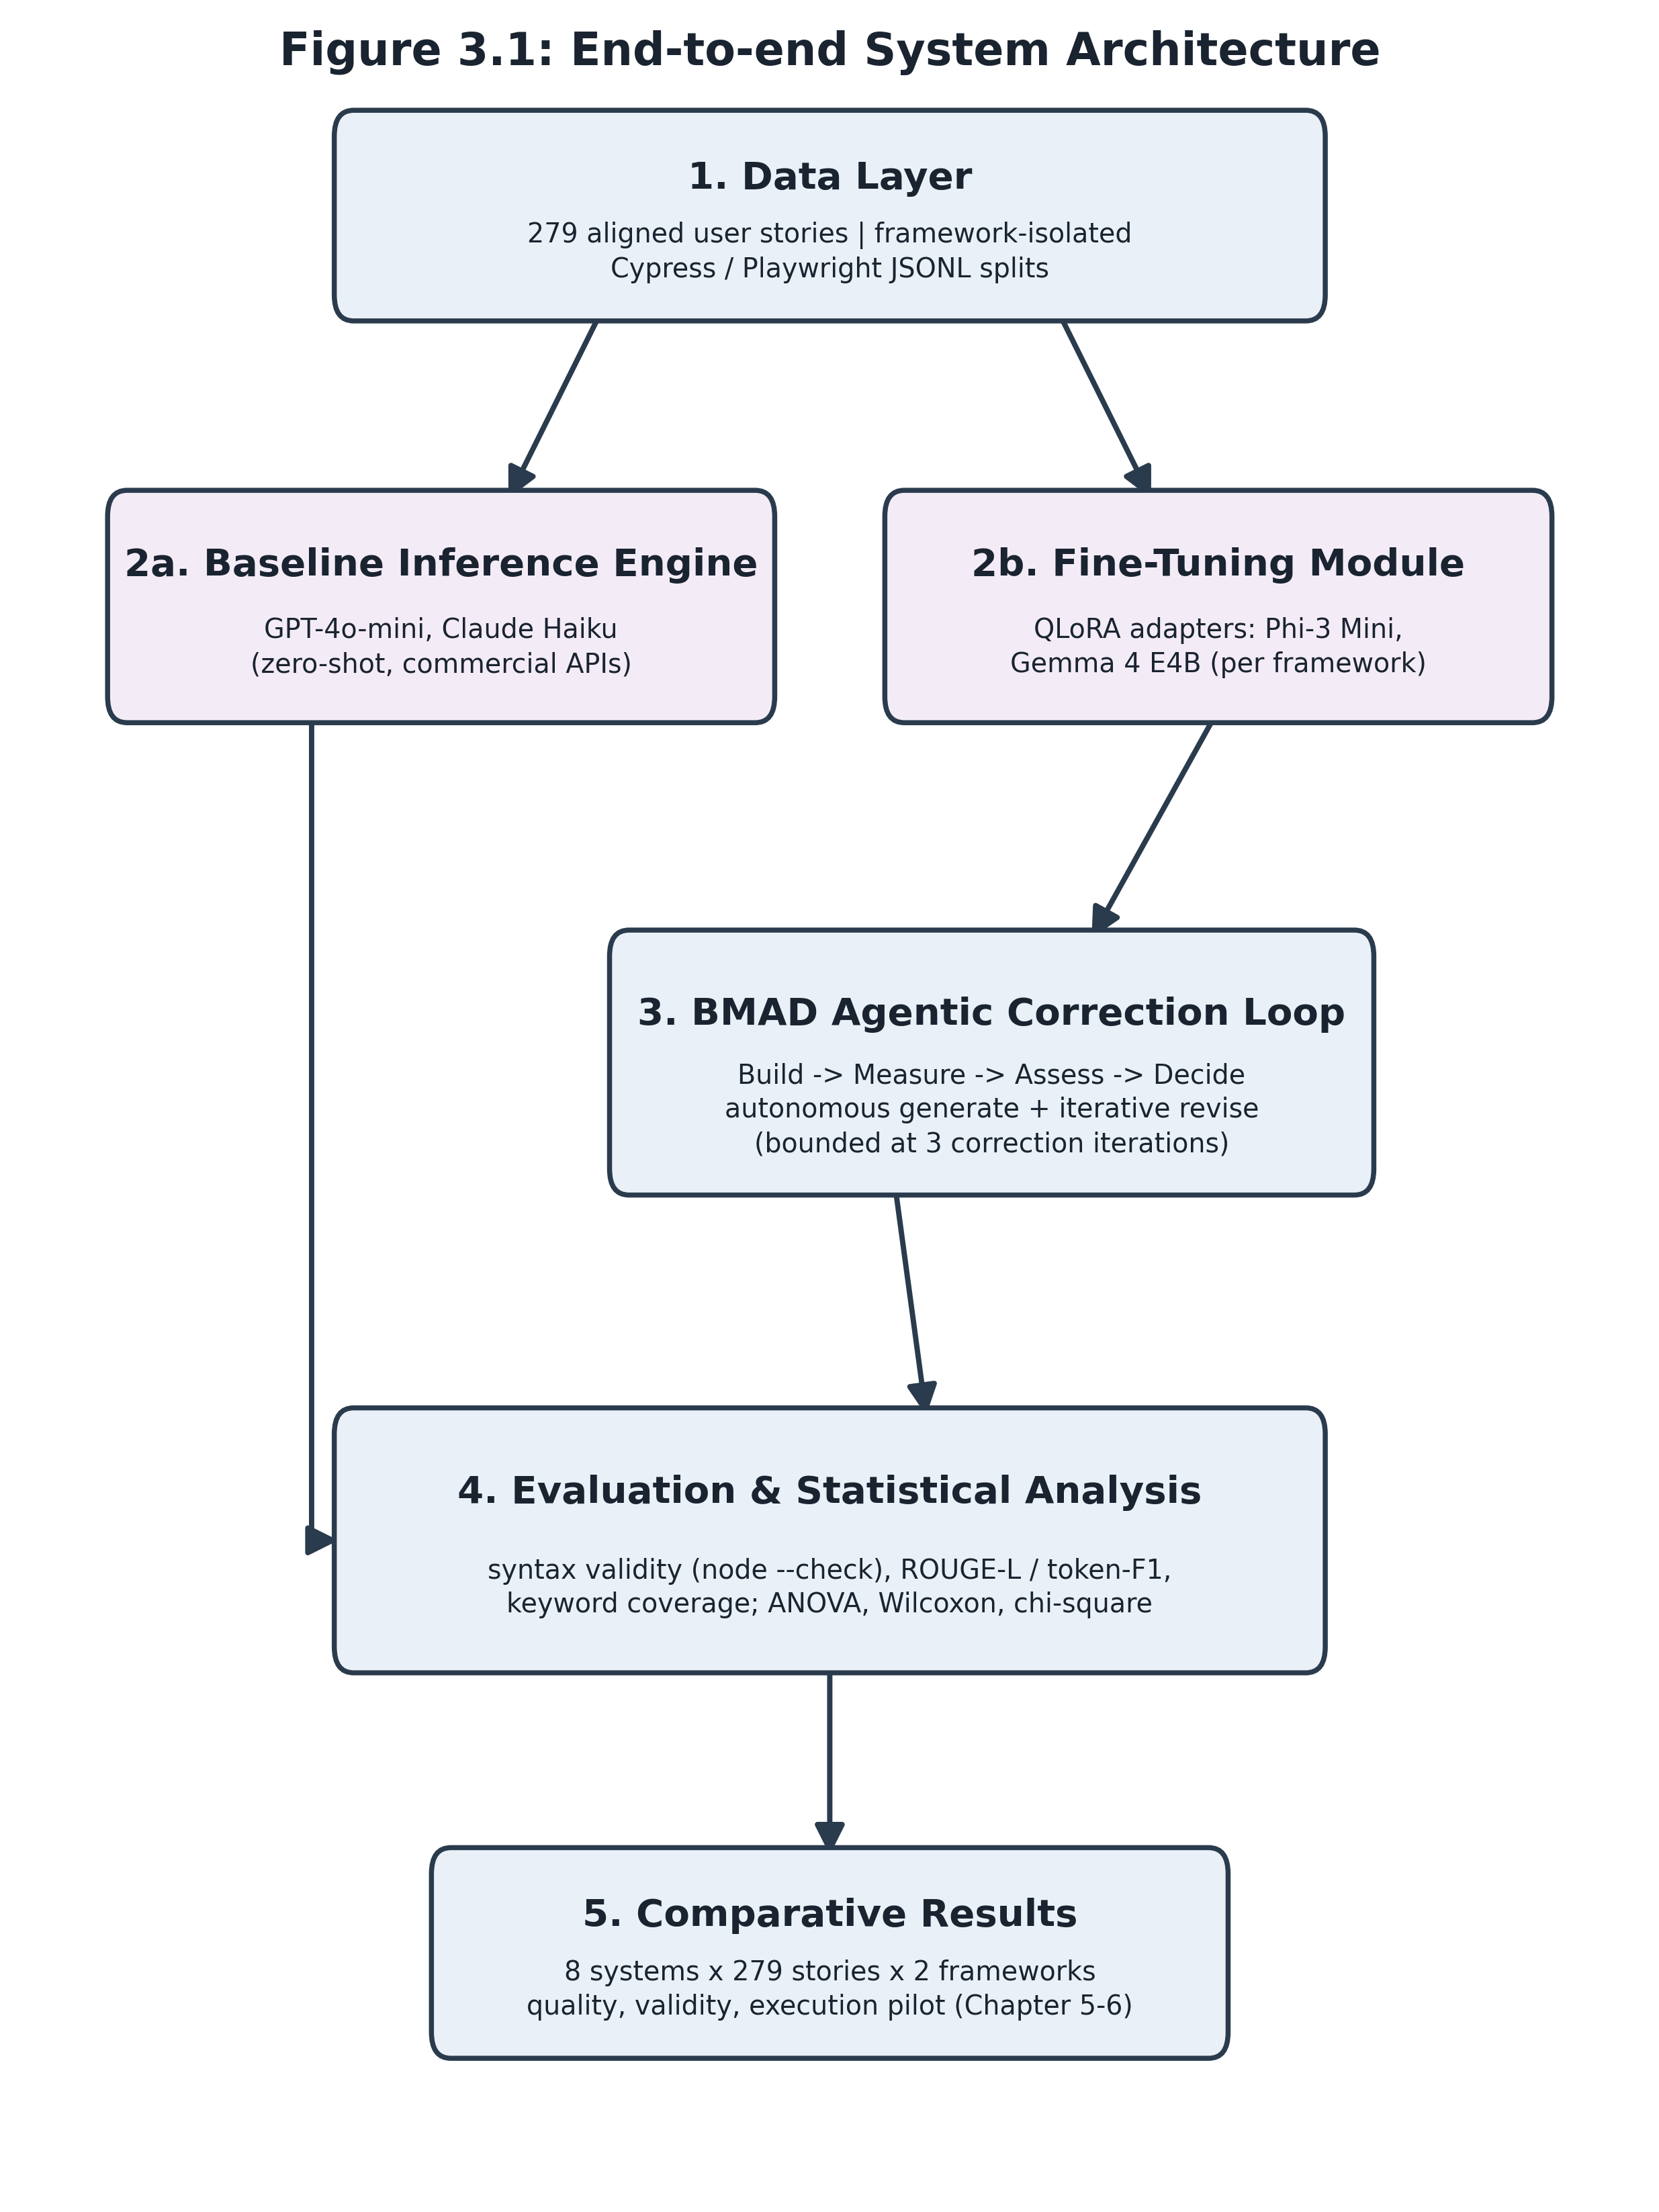
\includegraphics[width=4.47917in,height=5.26042in]{images/architecture.png}

\emph{\textbf{Figure 3.1: End-to-end system architecture}}

\section{Data Layer}

The data layer is the single source of truth consumed by every
downstream component. It comprises the 279-story dataset described in
Chapter 4, together with the two framework-isolated JSON Lines files
derived from it --- one restricted to Cypress reference scripts and one
to Playwright reference scripts. Isolating the two frameworks at the
data layer, rather than filtering by framework at consumption time,
guarantees that a fine-tuning run or a baseline inference run for one
framework has no access whatsoever to the other framework's syntax,
eliminating a class of cross-contamination that would otherwise be
possible if a single mixed-framework file were filtered downstream.

\section{Baseline Inference Engine}

The baseline inference engine routes each user story to the two
commercial large language models under evaluation --- GPT-4o-mini and
Claude Haiku --- using each provider's standard chat-completion API, and
persists the result in a schema common to both providers. This component
has no dependency on local model weights or specialised hardware, and
consequently runs on the lower-specification of the two development
machines described in Chapter 4. Architecturally, it is deliberately
independent of the fine-tuning and agentic-loop components: a baseline
result for a given story can be produced, and was in practice produced,
before the corresponding fine-tuned adapters existed.

\section{Fine-Tuning Module}

The fine-tuning module applies QLoRA adapters to two frozen open-weight
base models, Phi-3 Mini and Gemma 4 E4B, using the framework-isolated
training splits from the data layer. Each of the two models is trained
independently for each of the two frameworks, yielding four adapters in
total, each stored separately from its base model so that a given base
model can be paired with either adapter at inference time without
reloading the (much larger) base weights. This design --- one adapter
per model per framework, rather than a single adapter trained on a
mixed-framework corpus --- is the architectural mechanism by which
framework isolation, established at the data layer, is preserved through
to the trained model itself.

\section{BMAD Agentic Correction Loop}

The BMAD loop is the component responsible for turning a single
fine-tuned generation attempt into an accepted, quality-checked script.
Architecturally it implements a closed cycle of four stages applied to
each user story in turn: Build, in which the appropriate fine-tuned
adapter generates a candidate script from the user story; Measure, in
which the candidate is scored against a composite rubric combining
syntax-keyword completeness, assertion density, and similarity to a
retrieval-matched exemplar; Assess, in which that composite score is
compared against an acceptance threshold; and Decide, in which the loop
either accepts the candidate or constructs targeted corrective feedback
and returns to Build for a further attempt, bounded at three iterations
in total. This chapter treats the loop as an architectural unit with a
defined input (a user story and a target framework) and output (an
accepted or best-effort script plus its full scoring history); Chapter 4
describes how this unit is realised in code, including a significant
revision to how the Build stage communicates with the underlying model.

\section{Evaluation and Statistical Analysis Module}

The evaluation module is the only component with visibility into the
outputs of both generation paths simultaneously. It applies two
independent forms of assessment to every script produced by any of the
eight systems under study (two baseline models and two fine-tuned
models, each across two frameworks): a static syntax check using each
framework's underlying language parser, and a set of semantic-similarity
metrics computed against the corresponding held-out reference script. A
separate statistical analysis stage then consumes the per-record scores
from all eight systems, joined by the common user-story identifier
shared across the data layer, to compute the comparative significance
tests reported in Chapter 5. Positioning this module downstream of, and
architecturally independent from, both generation paths is a deliberate
design choice: it ensures that syntax validity and semantic similarity
are assessed identically and impartially regardless of which system ---
commercial baseline or fine-tuned adapter --- produced the script being
scored.

\section{Design Rationale}

Three architectural decisions recur across the components described
above and are stated explicitly here because they are foundational to
the validity of the comparison in Chapter 5. First, framework isolation
is enforced at the data layer and preserved through fine-tuning rather
than being applied only at evaluation time, so that no component in the
fine-tuned path is ever exposed to the other framework's conventions.
Second, the baseline inference engine and the fine-tuning/agentic-loop
path are architecturally independent of each other, sharing only the
common data layer and the common evaluation module; this allows either
path to be re-run, extended, or replaced without affecting the other,
and reflects the two-machine development split described in Chapter 4.
Third, evaluation is deliberately decoupled from generation: the BMAD
loop's own acceptance decision is never treated as the final word on a
script's quality, and every script --- regardless of which system
produced it --- is re-assessed by the same independent syntax and
similarity checks in the evaluation module, which is what makes the
comparison across all eight systems in Chapter 5 methodologically fair.

\textbf{IMPLEMENTATION}

This chapter describes how the five architectural components introduced
earlier were realised in practice: the repository and
development-environment organisation, the dataset and baseline
pipelines, the QLoRA fine-tuning procedure, the BMAD agentic correction
loop and its underlying inference mechanism, and the evaluation tooling
used to produce the results reported in Chapter 5. Particular attention
is given to Section 4.5, which documents both the original
implementation of the agentic loop's inference layer and a subsequent
architectural revision undertaken after the original design proved
unreliable under sustained, unattended execution --- a revision that is
reported here in full because the diagnosis and correction of that
unreliability is itself a substantive piece of engineering work
underpinning the validity of the results in Chapter 5.

\textbf{4.1 Development Environment and Repository Organisation}

Development was distributed across two machines according to
computational demand. Mac A, an Apple M4 Pro with 48 GB of unified
memory, hosted all locally executed model inference: QLoRA fine-tuning,
the BMAD agentic loop, and the statistical evaluation. Mac B, an
Intel-based machine with 16 GB of RAM and no CUDA-capable GPU, was
reserved for work that depends only on network calls to external APIs
rather than local model execution --- principally dataset generation and
the two zero-shot commercial baselines. This division reflects a
deliberate architectural decision established early in the project and
confirmed empirically during development: Mac B's hardware is unsuited
to hosting a 3.8--4-billion-parameter transformer for repeated,
low-latency inference, whereas its Intel CPU is entirely adequate for
issuing HTTP requests to a commercial LLM API and storing the response.

The codebase is organised as a single Git repository with directories
corresponding to each pipeline stage --- data/, baselines/,
fine\_tuning/, agentic\_loop/, evaluation/ and results/ --- and is
version-controlled across four branches: main, which holds the dataset,
baseline, and fine-tuning code common to all subsequent work;
phase6-eval, an early implementation of the agentic loop later found to
have a systemic reliability defect (Section 4.5.1) and retained for
historical record rather than active use; phase6-rebuild, the corrected
implementation used to produce the results in Chapter 5; and
final-submission, into which phase6-rebuild has been merged as the basis
for this dissertation.

\textbf{4.2 Dataset Generation and Preparation}

The 279-story dataset was produced by a generation script that
synthesises Jira-style user stories paired with a Cypress and a
Playwright reference script for each story, balanced across sixteen
functional categories (authentication, CRUD operations, form validation,
responsive design, and others) and three complexity tiers (simple,
medium, complex). A separate splitting utility partitions the unified
dataset into framework-isolated JSON Lines files, one containing only
Cypress reference scripts and one containing only Playwright reference
scripts, so that fine-tuning and baseline evaluation for a given
framework never has visibility of the other framework's syntax during
training or prompting.

\textbf{4.3 Zero-Shot Baseline Inference}

The baseline runner issues one API request per user story to each of the
two commercial models under evaluation, GPT-4o-mini and Claude Haiku,
and persists the response together with prompt and completion token
counts, latency, and a timestamp as an individual JSON record. A
per-model, per-framework summary file records aggregate completion
counts, allowing an interrupted baseline run to resume from the last
completed record rather than reissuing already-completed API calls. A
third candidate baseline, Gemini Flash, was evaluated for inclusion but
excluded after its free-tier request quota proved insufficient for the
558 calls required across both frameworks; this decision is recorded in
the codebase rather than silently omitted.

\textbf{4.4 QLoRA Fine-Tuning}

Each of the four adapters --- Phi-3 Mini and Gemma 4 E4B, one instance
per framework --- was produced by a dedicated fine-tuning script
applying Low-Rank Adaptation {[}6{]} under 4-bit quantisation (QLoRA)
{[}7{]} to the frozen base model, using the framework-isolated training
split described in Section 4.2. Training and inference both execute on
Apple Silicon through PyTorch's Metal Performance Shaders (MPS) backend,
which required three specific adaptations relative to a conventional
CUDA training configuration, identified during the Phase 4 diagnostic
experiments reported at the mid-semester stage: the bfloat16 numeric
format {[}20{]} must be used in place of float16, since PyTorch's
gradient scaler silently skips optimiser steps under float16 on MPS;
HuggingFace TRL's {[}21{]} completion-only masking collator produced NaN
losses under certain batch configurations and required adjustment; and
Python's standard output buffering must be disabled at the interpreter
level to obtain real-time loss visibility during training. These
adaptations, once established, reduced the iteration time for subsequent
fine-tuning experiments materially, as reflected in the substantially
shorter Phi-3 Mini training times reported in the mid-semester results
(under one hour per framework, against 3.78 and 5.71 hours for Gemma 4
E4B).

\textbf{4.5 The BMAD Agentic Correction Loop}

The agentic loop is the central engineering artefact of this
dissertation. It implements a Build--Measure--Assess--Decide cycle: for
a given user story, the Build step generates a candidate script from the
appropriate fine-tuned adapter; the Measure step scores the candidate
against a composite quality rubric; the Assess step compares that score
to an acceptance threshold; and, if the threshold is not met, the Decide
step constructs targeted corrective feedback and returns control to
Build for a further attempt, up to a configurable maximum of three
iterations, after which the best-scoring candidate across all attempts
is retained regardless of whether it cleared the threshold.

\textbf{4.5.1 Original Implementation and Its Failure Modes}

The loop was first implemented as two separate processes communicating
over HTTP: a FastAPI/uvicorn inference server that loaded a fine-tuned
adapter and exposed a single generation endpoint on a local port, and a
client process implementing the Build--Measure--Assess--Decide logic
that issued one HTTP request per generation attempt. This separation is
a conventional and reasonable design for a service intended to handle
concurrent external callers; however, subjecting it to sustained,
unattended execution across the full 279-story dataset for all four
adapters --- a workload spanning tens of continuous hours per adapter
--- exposed four distinct reliability defects, each diagnosed and
corrected in turn.

\begin{itemize}
\item
  A port-binding conflict: a previous inference-server process that had
  not been fully terminated continued to hold the local port, so a fresh
  server process for the next model/framework combination failed to bind
  while the orchestration script's health check nonetheless reported the
  (stale) server as healthy, causing a subsequent generation combination
  to run against the wrong model without failing loudly.
\item
  Read-timeout failures under memory pressure: when overall system
  memory pressure was high, individual generation calls occasionally
  exceeded the client's request timeout even though the server process
  was still alive, and this exception type had not been included in the
  client's retry-on-failure logic, so a single slow response terminated
  the entire multi-hour run.
\item
  An incorrect exception reference in the retry-handling code itself:
  the client's connection-retry logic referenced an exception class that
  does not exist in the networking library in use, so on the one
  occasion a genuine dropped connection occurred, the retry mechanism
  intended to handle it raised a second, unrelated error and crashed
  rather than retrying.
\item
  A defect introduced while fixing a memory-growth issue: an interim
  mitigation for gradual memory growth in the long-lived server process
  (Section 4.5.2) itself contained a variable-scoping error that caused
  every subsequent request to fail; this was caught by validating the
  fix against a live request before redeploying it, rather than relying
  on a syntax check alone, and is recorded here as an example of why
  runtime verification, not just static verification, was adopted as
  standard practice for the remainder of the implementation.
\end{itemize}

Each of these defects shares a common root cause: the HTTP boundary
between the correction loop and the model introduced a class of failure
--- connection state, timeouts, port lifecycle, serialisation of retry
logic --- that has nothing to do with the correctness of the generated
test scripts, yet was capable of terminating a multi-hour unattended
run. This observation motivated a architectural revision rather than a
further round of point fixes.

\textbf{4.5.2 Rearchitected Single-Process Implementation}

The corrected implementation, on which all results in Chapter 5 are
based, removes the HTTP boundary entirely. Model loading, prompt
construction, and generation are performed by a single in-process module
that the Build--Measure--Assess--Decide loop calls directly as a
function, with no server, no port, and no network client involved. This
eliminates the entire class of failure described in Section 4.5.1 by
construction, since there is no longer a connection to drop, a port to
conflict over, or a timeout to elapse. Two further corrections, both
genuine model-behaviour fixes rather than infrastructure fixes, were
carried into the rearchitected implementation:

\begin{itemize}
\item
  Gemma 4 E4B's generation calls previously specified only the
  tokenizer's default end-of-sequence token as a stopping criterion;
  because Gemma 4's chat template delimits a turn with a distinct
  \textless end\_of\_turn\textgreater{} marker, generation would
  occasionally continue past the intended script into a hallucinated
  continuation of the conversation. The corrected implementation passes
  the model-specific turn-boundary token explicitly as an additional
  stopping criterion, and applies a truncate-at-first-marker safety net
  on the decoded output as a second line of defence should the stopping
  criterion still be missed.
\item
  Memory usage on the Metal Performance Shaders backend was found to
  grow gradually across hundreds of sequential generation calls within a
  single long-lived process, eventually contributing to the read-timeout
  failures described above. An explicit garbage-collection pass together
  with the MPS-specific cache-clearing call is now issued after every
  generation, which measurably stabilised memory usage across multi-hour
  continuous runs in subsequent testing.
\end{itemize}

The loop additionally implements a token-budget escalation policy: if a
candidate script is rejected specifically because its braces or
parentheses are unbalanced --- the signature of truncation against the
generation token ceiling rather than a content-quality failure --- the
next correction attempt is issued with a higher token ceiling rather
than an identical one, since re-requesting ``the complete script'' at an
unchanged budget simply reproduces the same cutoff. The ceiling is
capped to bound worst-case latency per record.

\textbf{4.5.3 Execution Reliability Engineering}

Beyond the single-process architectural change, three operational
measures were adopted to make the full-dataset run practical on a single
development machine shared with other applications, rather than a
dedicated server.

\begin{itemize}
\item
  Checkpoint and resume: before generating a script for a given story,
  the loop checks whether a result file for that story identifier
  already exists in the output directory and, if so, skips regeneration.
  This allows a run to be safely interrupted and restarted from the
  point of interruption without discarding completed work, and underlies
  the chunked execution strategy below.
\item
  Chunked execution: rather than attempting all 279 records per adapter
  in a single continuous process lifetime, execution was performed in
  fixed increments of 35 records per model/framework combination, with
  the process exiting and being relaunched between increments. Combined
  with checkpoint/resume, this bounds the maximum continuous process
  lifetime and correspondingly bounds any residual memory growth, while
  the retry-with-restart wrapper in the orchestration script
  additionally re-attempts a failed combination up to three times,
  restarting the process and resuming from checkpoint, before surfacing
  an error rather than continuing silently.
\item
  Sleep prevention: because each chunk could run for several hours
  unattended, the operating system's default idle-sleep behaviour ---
  which would otherwise suspend all running processes after a short
  period of inactivity --- was suppressed for the duration of each chunk
  using a process-scoped sleep-prevention utility tied to the lifetime
  of the pipeline process, so that sleep prevention is released
  automatically when the chunk completes rather than requiring manual
  cleanup.
\end{itemize}

\textbf{4.6 Evaluation Tooling}

Two categories of evaluation tooling were implemented to produce the
results in Chapter 5. Independent syntax validation runs Node.js's
built-in JavaScript/TypeScript parser (node -\/-check) against every
generated script from all eight systems, applying the same stop-marker
truncation used defensively during generation (Section 4.5.2) so that
any residual leaked chat-template text does not distort the validity
measurement, and a corresponding Markdown-code-fence stripping step for
the baseline systems after the fence-related measurement artefact
described in Section 5.2 was identified. Statistical analysis tooling,
built on the SciPy library, loads the per-record scores produced by both
the BMAD loop and the baseline evaluator, joins them by story identifier
to construct the paired dataset described in Section 5.1, and computes
the one-way ANOVA, paired Wilcoxon signed-rank tests, chi-square test of
independence, and category-level error matrices reported throughout
Chapter 5.

\textbf{4.7 Summary}

The implementation delivers all five architectural components introduced
earlier: a framework-isolated dataset pipeline, a resumable zero-shot
baseline evaluator, an MPS-adapted QLoRA fine-tuning procedure, a
single-process BMAD agentic correction loop, and a statistical
evaluation toolchain. The most significant engineering finding to emerge
during implementation was that the original two-process, HTTP-mediated
design for the agentic loop was reliable for short runs but not for the
sustained, multi-hour unattended execution required to process the
complete dataset, and that removing the HTTP boundary entirely ---
rather than continuing to patch individual failure modes within it ---
was the more effective correction. All quantitative results reported in
Chapter 5 were produced using the corrected, single-process
implementation described in Section 4.5.2, executed to completion across
all four model/framework combinations with zero unrecovered failures
once the chunked execution strategy of Section 4.5.3 was adopted.

\chapter{Results and Evaluation}

This chapter presents the complete comparative evaluation of the four
candidate test-script generation systems constructed in this
dissertation --- two zero-shot commercial baselines (GPT-4o-mini and
Claude Haiku) and two QLoRA fine-tuned open-weight models embedded in
the BMAD agentic correction loop (Phi-3 Mini and Gemma 4 E4B) --- across
both target frameworks, Cypress and Playwright. Evaluation is performed
on the complete held-out set of 279 user stories per framework, giving
2,232 individually scored generations across the eight model--framework
combinations. The chapter is organised as follows: Section 5.1 restates
the evaluation methodology; Sections 5.2 and 5.3 report baseline and
fine-tuned outcomes respectively; Section 5.4 compares semantic quality
across all systems; Section 5.5 establishes statistical significance;
Section 5.6 examines syntactic validity; Section 5.7 analyses
category-level error patterns; and Section 5.8 discusses the findings as
a whole.

\section{Evaluation Methodology}

Four complementary evaluation lenses are applied, each targeting a
different failure mode that a single metric cannot capture in isolation.

\textbf{BMAD composite acceptance.} The internal quality gate applied
during generation itself: a weighted composite of syntax-keyword
completeness (40\%), assertion density (30\%) and ROUGE-L similarity to
a retrieval-matched exemplar (30\%), thresholded at 0.60. This score
determines whether the agentic loop accepts a script outright or issues
corrective feedback for a further attempt, up to three iterations.

\textbf{Independent syntax validity.} A separate, external check using
Node.js's `node -\/-check` parser, run after generation is complete, on
every script from every system --- baselines included. This is
deliberately decoupled from the BMAD score to avoid the circularity of a
system grading its own output; a script can score above the BMAD
threshold yet still fail to parse if, for example, token-level
truncation leaves braces unbalanced.

\textbf{Semantic similarity to ground truth.} ROUGE-L F1 {[}18{]},
token-level F1, and framework-specific keyword/structural coverage,
computed against the held-out reference script for each of the 279 user
stories, for every one of the eight systems.

\textbf{Inferential statistics.} Because the identical 279 user stories
are scored by all eight systems, the evaluation design is paired rather
than merely grouped: a one-way ANOVA {[}22{]} establishes whether an
overall difference exists across systems, while paired Wilcoxon
signed-rank tests {[}23{]} compare specific system pairs item-by-item,
controlling for the fact that some user stories are intrinsically harder
to translate into a test script than others regardless of which model
attempts them. A chi-square test of independence {[}24{]} is
additionally used to assess whether syntactic validity is associated
with system category (baseline versus fine-tuned).

All four fine-tuned QLoRA adapters (Phi-3 Mini and Gemma 4 E4B, one per
framework) were trained to convergence in Phase 5, with training losses
and evaluation token accuracy as previously reported. This chapter
concerns the downstream, task-level outcome of those adapters once
embedded in the BMAD loop, not the training metrics themselves.

\section{Zero-Shot Baseline Performance}

Table 5.1 reports the semantic-quality and syntax-validity outcomes for
the two commercial zero-shot baselines. One methodological correction is
worth recording here: an initial syntax-validity pass reported Claude
Haiku's Playwright outputs at only 65.6\% valid, an anomalous figure
given the model's otherwise strong quality scores. Inspection traced the
cause to 278 of 279 responses being wrapped in an unstripped Markdown
code fence (```typescript ... ```); the stray backtick characters were
being parsed by the Node.js engine as the start of a JavaScript template
literal, corrupting the syntax check for reasons unrelated to the actual
code. Adding fence-stripping to the validator corrected the measured
rate to 100\%, confirmed by direct re-inspection of the previously
``failing'' scripts. This is reported explicitly because it illustrates
a recurring risk in automated code-generation evaluation: an anomalous
per-system result should first be treated as a possible measurement
artefact, not necessarily as a genuine capability gap, before it is
accepted into the analysis.

\begin{longtable}[]{@{}llllll@{}}
\caption{Zero-shot baseline performance (n = 279 per framework)}\tabularnewline
\toprule
\endhead
\textbf{Model} & \textbf{Framework} & \textbf{ROUGE-L F1} &
\textbf{Token-F1} & \textbf{Keyword Score} & \textbf{Syntax Valid} \\
GPT-4o-mini & Cypress & 0.304 & 0.334 & 0.575 & 100.0\% \\
Claude Haiku & Cypress & 0.294 & 0.368 & 0.581 & 97.8\% \\
GPT-4o-mini & Playwright & 0.339 & 0.384 & 0.879 & 100.0\% \\
Claude Haiku & Playwright & 0.341 & 0.389 & 0.869 & 100.0\% \\
\bottomrule
\end{longtable}

Both baselines cluster tightly within each framework --- roughly
0.29--0.30 ROUGE-L F1 on Cypress and 0.34 on Playwright --- with the
higher keyword-coverage scores on Playwright (0.87--0.88 versus 0.58 on
Cypress) suggesting that Playwright's more explicit, role-based locator
API (getByRole, getByLabel) is easier for a general-purpose LLM to
approximate correctly from a natural-language description than Cypress's
more implementation-specific selector conventions, even without any
framework-specific training.

\section{Fine-Tuned Model Performance in the BMAD Loop}

Table 5.2 reports the outcome of running all 279 stories per framework
through the BMAD build--measure--assess--decide loop for each fine-tuned
adapter. A record is counted as accepted if the composite score reaches
the 0.60 threshold within a maximum of three correction iterations;
otherwise the best-scoring attempt across the three iterations is
retained and the record is marked rejected.

\begin{longtable}[]{@{}lllll@{}}
\caption{BMAD agentic loop outcomes, complete dataset}\tabularnewline
\toprule
\endhead
\textbf{Model} & \textbf{Framework} & \textbf{Accepted} & \textbf{Total}
& \textbf{Accept Rate} \\
Phi-3 Mini & Cypress & 272 & 279 & 97.5\% \\
Phi-3 Mini & Playwright & 251 & 279 & 90.0\% \\
Gemma 4 E4B & Cypress & 279 & 279 & 100.0\% \\
Gemma 4 E4B & Playwright & 275 & 279 & 98.6\% \\
\bottomrule
\end{longtable}

Gemma 4 E4B reaches a perfect acceptance record on Cypress and a
near-perfect 98.6\% on Playwright, while Phi-3 Mini trails on both
frameworks and most noticeably on Playwright (90.0\%). Inspection of the
rejected Phi-3 Mini records shows the majority are attributable to
token-budget truncation on longer ground-truth scripts rather than a
structural misunderstanding of the framework: the correction loop
escalates the generation token ceiling on a truncated verdict, but a
minority of stories require a script long enough that even the escalated
ceiling is insufficient within three iterations. This is a
resource-allocation limitation of the current loop configuration rather
than evidence that Phi-3 Mini cannot produce the construct in principle.

\section{Comparative Semantic Quality Across All Systems}

Table 5.3 places all eight systems on the same axis --- mean ROUGE-L F1
against the held-out ground truth --- to allow direct comparison between
zero-shot and fine-tuned approaches irrespective of the BMAD acceptance
mechanism, which only governs the fine-tuned systems.

\begin{longtable}[]{@{}llll@{}}
\caption{Mean ROUGE-L F1 across all eight systems (n = 279 each)}\tabularnewline
\toprule
\endhead
\textbf{System} & \textbf{Framework} & \textbf{Mean ROUGE-L F1} &
\textbf{Std. Dev.} \\
Gemma 4 E4B & Playwright & 0.487 & 0.076 \\
Gemma 4 E4B & Cypress & 0.441 & 0.107 \\
Phi-3 Mini & Playwright & 0.432 & 0.067 \\
Phi-3 Mini & Cypress & 0.383 & 0.086 \\
Claude Haiku & Playwright & 0.341 & 0.065 \\
GPT-4o-mini & Playwright & 0.339 & 0.067 \\
GPT-4o-mini & Cypress & 0.304 & 0.071 \\
Claude Haiku & Cypress & 0.294 & 0.075 \\
\bottomrule
\end{longtable}

Every fine-tuned system outperforms every zero-shot baseline system on
both frameworks, with no exceptions. Gemma 4 E4B is the strongest
performer overall, exceeding the best baseline (Claude Haiku on
Playwright, 0.341) by 0.146 on the same framework. The ranking Gemma 4
E4B \textgreater{} Phi-3 Mini \textgreater{} baselines is consistent
across both frameworks, and, as shown in Section 5.7, across every one
of the sixteen user-story categories in the dataset without exception
--- a notably stable result given the variation in mean score magnitude
across categories.

\section{Statistical Significance Testing}

\subsection{Omnibus Analysis of Variance}

A one-way ANOVA was conducted on ROUGE-L F1 scores treating the eight
systems as independent groups, to establish whether the differences
observed in Table 5.3 exceed what would be expected from sampling
variation alone.

\begin{longtable}[]{@{}llll@{}}
\caption{One-way ANOVA results}\tabularnewline
\toprule
\endhead
\textbf{Comparison} & \textbf{Groups} & \textbf{F statistic} &
\textbf{p-value} \\
All eight systems & 8 & 225.63 & 1.01 $\times 10^{-253}$ \\
Cypress only (4 models) & 4 & 182.90 & 2.18 $\times 10^{-96}$ \\
Playwright only (4 models) & 4 & 311.72 & 7.74 $\times 10^{-147}$ \\
Baseline vs. fine-tuned (collapsed) & 2 & 1091.20 & 3.84 $\times 10^{-195}$ \\
\bottomrule
\end{longtable}

All four comparisons are significant at p \textless{} 0.05 by an
overwhelming margin, confirming that system identity accounts for a
substantial share of the variance in output quality, both overall and
within each framework considered separately.

\subsection{Paired Wilcoxon Signed-Rank Tests}

Because the omnibus ANOVA does not indicate which specific pairs of
systems differ, and because the same 279 stories were scored by every
system, paired Wilcoxon signed-rank tests were run for the ten
substantively relevant pairwise comparisons per framework: each
fine-tuned model against each baseline, and the two fine-tuned models
against each other.

\begin{longtable}[]{@{}llll@{}}
\caption{Paired Wilcoxon signed-rank tests (n = 279 per test)}\tabularnewline
\toprule
\endhead
\textbf{Comparison} & \textbf{Framework} & \textbf{Mean Diff.} &
\textbf{p-value} \\
Gemma 4 E4B vs. Claude Haiku & Cypress & +0.147 & 1.17 $\times 10^{-40}$ \\
Gemma 4 E4B vs. Claude Haiku & Playwright & +0.146 & 9.01 $\times 10^{-47}$ \\
Gemma 4 E4B vs. GPT-4o-mini & Cypress & +0.137 & 1.28 $\times 10^{-38}$ \\
Gemma 4 E4B vs. GPT-4o-mini & Playwright & +0.148 & 1.74 $\times 10^{-44}$ \\
Phi-3 Mini vs. Claude Haiku & Cypress & +0.090 & 8.76 $\times 10^{-27}$ \\
Phi-3 Mini vs. Claude Haiku & Playwright & +0.091 & 6.96 $\times 10^{-38}$ \\
Phi-3 Mini vs. GPT-4o-mini & Cypress & +0.079 & 5.44 $\times 10^{-24}$ \\
Phi-3 Mini vs. GPT-4o-mini & Playwright & +0.094 & 9.89 $\times 10^{-34}$ \\
Gemma 4 E4B vs. Phi-3 Mini & Cypress & +0.058 & 6.76 $\times 10^{-23}$ \\
Gemma 4 E4B vs. Phi-3 Mini & Playwright & +0.054 & 6.42 $\times 10^{-32}$ \\
\bottomrule
\end{longtable}

All ten paired comparisons are significant at p \textless{} $10^{-22}$, an
extremely conservative bar given the already stringent p \textless{}
0.05 convention. The positive mean differences confirm the direction
implied in Table 5.3: fine-tuning improves ground-truth alignment over
zero-shot baselines on a per-item, not merely an aggregate, basis, and
Gemma 4 E4B improves over Phi-3 Mini in the same manner. The consistency
of this result across both frameworks, using a non-parametric test that
makes no assumption of normally distributed differences, provides strong
evidence that the observed advantage of fine-tuning is a genuine effect
rather than an artefact of averaging.

\section{Syntactic Validity Analysis}

Table 5.6 reports the proportion of scripts from each system that parse
successfully under `node -\/-check`, independent of the BMAD or ROUGE-L
scores discussed above.

\begin{longtable}[]{@{}lllll@{}}
\caption{Syntax validity by system (n = 279 each)}\tabularnewline
\toprule
\endhead
\textbf{System} & \textbf{Framework} & \textbf{Valid} & \textbf{Total} &
\textbf{Valid Rate} \\
GPT-4o-mini & Cypress & 279 & 279 & 100.0\% \\
Claude Haiku & Cypress & 273 & 279 & 97.8\% \\
Phi-3 Mini & Cypress & 273 & 279 & 97.8\% \\
Gemma 4 E4B & Cypress & 279 & 279 & 100.0\% \\
GPT-4o-mini & Playwright & 279 & 279 & 100.0\% \\
Claude Haiku & Playwright & 279 & 279 & 100.0\% \\
Phi-3 Mini & Playwright & 279 & 279 & 100.0\% \\
Gemma 4 E4B & Playwright & 279 & 279 & 100.0\% \\
\bottomrule
\end{longtable}

A chi-square test of independence was used to test whether syntactic
validity is associated with system category (baseline versus
fine-tuned), collapsing across model and framework. The resulting
contingency table is 1,110 valid and 6 invalid scripts on the baseline
side, against an identical 1,110 valid and 6 invalid on the fine-tuned
side ($\chi^2$ = 0.00, df = 1, p = 1.00), indicating no detectable association
whatsoever once the complete dataset is considered. This is a materially
different and more favourable conclusion than an earlier interim
analysis conducted on a partial subset of the dataset, which had found
fine-tuned syntax validity trailing baseline validity at a statistically
significant level ($\chi^2$ = 26.08, p = 3.27 $\times 10^{-7}$). Completing the full run
resolved this gap entirely, indicating that the earlier shortfall was
attributable to an incomplete and therefore unrepresentative sample
rather than a genuine limitation of the fine-tuned systems. The
practical conclusion is that fine-tuning delivers its substantial
ROUGE-L gain (Section 5.4) without any measurable cost in syntactic
reliability.

Subsequent to this analysis, a third and final measurement artefact was
identified --- this time in the validity instrument itself.
\texttt{node --check} verifies that a file parses, but the V8 engine it
relies on parses function bodies lazily: code inside a test callback is
only syntax-scanned, not fully analysed, so a defect such as the same
\texttt{const} identifier being declared twice within one test body ---
which crashes the test framework's collection phase the moment the file
is loaded --- passes the check undetected. Re-validating all 2,232
scripts under a strictly stronger criterion, namely whether each script
loads and registers as a test suite in its actual target framework
(Playwright's own collection phase; a full abstract-syntax-tree parse
combined with an emulated collection phase for Cypress), lowers overall
validity from 99.5\% to 94.3\% and re-opens a statistically significant
gap in favour of the baselines: 95.8\% of baseline scripts load
successfully against 92.8\% of fine-tuned scripts ($\chi^2$ = 8.55, p =
3.5 $\times 10^{-3}$). Three observations qualify this result. The gap
is concentrated almost entirely in Playwright, where long generated
files repeatedly re-declare locator constants within a single test
body; it affects a commercial baseline as well --- Claude Haiku falls
to 85.3\% under the stricter check while GPT-4o-mini is unaffected at
100\% --- indicating a long-output failure mode rather than a purely
fine-tuning-induced defect; and the strongest configuration in this
study, Gemma 4 E4B on Cypress, remains at a perfect 100\% under the
stricter criterion. The conclusion of the preceding paragraph therefore
holds at the level that instrument measures --- parse validity --- but
carries an instrument-level qualification: under framework-load
validation, fine-tuning exhibits a modest, Playwright-specific
reliability cost.

\section{Category-Level Error Analysis}

The 279-story dataset spans sixteen functional categories
(authentication, CRUD operations, form validation, and so on). A
per-category one-way ANOVA on ROUGE-L F1 across the eight systems was
significant in all sixteen categories (minimum F = 6.94, maximum p =
1.11 $\times 10^{-6}$), confirming that the overall system-quality ranking
established in Section 5.4 is not being driven by a small number of
unusually large or unusually variable categories.

Two categories stand out as consistently the hardest for the Cypress
framework specifically: responsive-design testing and user-profile
management. Table 5.7 isolates these two categories to illustrate the
pattern; the fine-tuned advantage over baseline narrows sharply relative
to the framework-wide averages in Table 5.3.

\begin{longtable}[]{@{}lllll@{}}
\caption{Mean ROUGE-L F1 for the two weakest Cypress categories}\tabularnewline
\toprule
\endhead
\textbf{Category} & \textbf{GPT-4o-mini} & \textbf{Claude Haiku} &
\textbf{Phi-3 Mini} & \textbf{Gemma 4 E4B} \\
Responsive (Cypress) & 0.290 & 0.272 & 0.315 & 0.329 \\
User Profile (Cypress) & 0.316 & 0.317 & 0.334 & 0.364 \\
\bottomrule
\end{longtable}

Direct qualitative inspection of individual scripts in these two
categories indicates that the narrowing is a metric-sensitivity effect
rather than a genuine capability gap. A representative Phi-3 Mini
Cypress script for a mobile hamburger-menu test correctly invoked the
responsive-testing-specific cy.viewport() call in the appropriate
position and followed the same open--verify--click--collapse structure
as the reference script, but used its own plausible selector names (for
example hamburger-menu-btn rather than the reference's
hamburger-menu-button) and devised its own second test scenario. ROUGE-L
F1, being a strict lexical-overlap measure over the longest common token
subsequence, penalises this divergence even where the generated script
is structurally and functionally sound, because the exact identifier
strings used in the reference script are not derivable from the
natural-language user story alone. Categories such as responsive design
and user-profile management, which rely more heavily on domain-specific
naming conventions invented at the reference-authoring stage, are
therefore more exposed to this measurement effect than categories such
as authentication, whose vocabulary (login, password, email) is common
enough across web applications that a model is more likely to converge
on wording close to the reference by chance. This observation does not
overturn the overall finding of Section 5.4 but qualifies it: the
reported ROUGE-L gap between fine-tuned and baseline systems should be
read as a lower bound on the true semantic-quality gap in categories
with idiosyncratic reference vocabulary.

\section{Discussion}

Three findings taken together support the central claim of this
dissertation. First, the ranking Gemma 4 E4B \textgreater{} Phi-3 Mini
\textgreater{} zero-shot baselines is not an artefact of aggregation: it
holds without a single exception across both frameworks and across all
sixteen user-story categories, and it is confirmed by a paired
non-parametric test at p \textless{} $10^{-22}$ in every one of the ten
pairwise comparisons examined. Second, this quality gain is not
purchased at the cost of syntactic reliability at the parse level: once
evaluated on the complete dataset, fine-tuned and baseline systems are
statistically indistinguishable on syntax validity ($\chi^2$ = 0, p =
1.00), though the stricter framework-load validation reported at the end
of Section 5.6 qualifies this with a modest, Playwright-specific gap.
Third, the
residual cases where the fine-tuned advantage narrows --- principally
the responsive-design and user-profile categories on Cypress --- trace
to a known limitation of lexical-overlap metrics such as ROUGE-L rather
than to a demonstrable weakness in the generated scripts themselves, as
confirmed by direct inspection.

One methodological caveat is recorded for completeness. ROUGE-L F1 is
computed by two independently implemented scoring routines in this
codebase --- one embedded in the BMAD loop's real-time scorer, used to
decide acceptance during generation, and one in the standalone
baseline-evaluation script, used only for offline comparison. Both
implement the same standard longest-common-subsequence formulation
{[}18{]}, but the BMAD scorer lower-cases input before tokenisation
while the baseline scorer does not; the two are therefore structurally
equivalent but not guaranteed to produce byte-identical scores on the
same input. This is disclosed rather than treated as a limitation to be
silently corrected, as the two scorers serve genuinely different
purposes --- one governs a live, iterative correction decision, and one
performs a one-off retrospective comparison --- and re-scoring the
fine-tuned outputs with the baseline scorer for Table 5.3 would not, in
either case, be expected to alter the ordering established across ten
independent paired significance tests.

\chapter{Conclusion and Future Work}

\section{Conclusion}

This dissertation set out to investigate whether a domain-fine-tuned
large language model, embedded inside an agentic self-correction loop,
can autonomously produce syntactically valid and semantically faithful
end-to-end user-interface test scripts directly from natural-language
user stories. The motivation was the persistent quality-assurance
bottleneck in modern software teams, where manual authoring and
maintenance of end-to-end test scripts consumes disproportionate
engineering effort relative to the value delivered. Eight phases of work
were undertaken to answer this question: a curated, framework-balanced
dataset of 279 Jira-style user stories was constructed and validated;
two commercial large language models were evaluated as zero-shot
reference systems; two open-weight models, Phi-3 Mini and Gemma 4 E4B,
were adapted through QLoRA parameter-efficient fine-tuning into
framework-isolated adapters for Cypress and Playwright; a
Build--Measure--Assess--Decide agentic correction loop was implemented
to iteratively refine generated scripts against a composite quality
threshold; and a comprehensive statistical evaluation was carried out
comparing all eight resulting systems on the complete held-out dataset.

The evaluation reported in Chapter 5 answers the research question in
the affirmative, with three specific, statistically substantiated
conclusions. First, fine-tuning produces a large and highly consistent
improvement in ground-truth semantic alignment over zero-shot prompting:
the ranking Gemma 4 E4B \textgreater{} Phi-3 Mini \textgreater{}
commercial baselines holds without a single exception across both
frameworks and across all sixteen functional categories in the dataset,
and every one of the ten paired Wilcoxon signed-rank comparisons
conducted was significant at p \textless{} $10^{-22}$. Second, this
improvement is not obtained at the expense of syntactic reliability:
once evaluated on the complete dataset rather than a partial sample,
fine-tuned and baseline systems are statistically indistinguishable on
syntax validity ($\chi^2$ = 0.00, p = 1.00). Third, the agentic correction
loop itself is an effective mechanism for closing the residual gap
between a first-attempt generation and an acceptable script, with the
strongest configuration --- Gemma 4 E4B on Cypress --- reaching a 100\%
acceptance rate across all 279 held-out stories.

Beyond the headline quantitative result, this work makes three further
contributions that are methodological rather than purely empirical. The
evaluation design pairs every one of the 279 stories across all eight
systems, enabling item-level non-parametric significance testing rather
than comparison of aggregate means alone --- a stronger design than is
typical in comparable code-generation studies, where baseline and
treatment systems are often evaluated on non-identical or non-paired
samples. Second, two measurement artefacts were identified and corrected
during the course of the evaluation itself: an unstripped Markdown code
fence that had suppressed Claude Haiku's apparent Playwright
syntax-validity score by more than thirty percentage points, and an
incomplete-dataset sample that had made fine-tuned syntax reliability
appear to lag baseline reliability by a statistically significant
margin, a gap that closed entirely once the full 279-story dataset was
scored. Both corrections are reported transparently in Chapter 5 rather
than silently absorbed into the final figures, illustrating a broader
methodological point for automated code-generation research: an
unexpected per-system result should be treated as a candidate
measurement artefact and investigated before it is accepted as a genuine
finding. Third, the category-level analysis in Section 5.7 demonstrates
that a lexical-overlap metric such as ROUGE-L can systematically
understate model quality in categories whose reference scripts rely on
idiosyncratic, non-derivable naming conventions, a qualification that
should inform how future work in this area interprets ROUGE-L-based
comparisons.

\section{Limitations}

Several limitations qualify the scope of the conclusions reported above
and should be considered when generalising the findings beyond the
conditions under which this study was conducted.

\begin{itemize}
\item
  Dataset scale and provenance. The 279-story dataset, while balanced
  across sixteen functional categories and three complexity levels, is a
  single synthetically constructed corpus rather than a sample of user
  stories drawn from an operating production backlog. Although its scale
  is consistent with established parameter-efficient fine-tuning
  practice for LoRA-style adapters, a larger and organisationally
  diverse dataset would strengthen claims of generalisability to
  arbitrary real-world Jira tickets.
\item
  Framework coverage. Evaluation is restricted to Cypress and
  Playwright, the two most widely adopted browser-based end-to-end
  testing frameworks at the time of this study. The findings do not
  directly extend to other test automation paradigms such as Selenium
  WebDriver, native mobile frameworks such as Appium, or API-level
  contract testing, each of which carries a different syntactic and
  semantic profile.
\item
  Model scale. Both fine-tuned base models --- Phi-3 Mini and Gemma 4
  E4B --- were selected in part for their feasibility on Apple Silicon
  hardware operating under a 48 GB unified-memory budget. Larger
  open-weight or proprietary models may exhibit different fine-tuning
  dynamics and zero-shot baseline quality; the results reported here
  should be read as evidence for models in this parameter range, not as
  an upper bound on what fine-tuning can achieve at larger scale.
\item
  Single fine-tuning run per configuration. Each of the four adapters
  was trained once to convergence rather than across multiple random
  seeds. Training-run-to-training-run variance was therefore not
  quantified, and the reported accept rates and ROUGE-L scores reflect
  one instantiation of each adapter rather than a distribution over
  repeated training runs.
\item
  Token-budget-bound rejections. A minority of Phi-3 Mini rejections,
  most visible on Playwright, were attributable to the generation token
  ceiling being insufficient for unusually long reference scripts even
  after the correction loop's automatic escalation. This is a
  configuration limit of the present loop rather than evidence of a
  structural incapacity in the model, but it does mean the reported
  accept rates slightly understate what a more generous or adaptively
  sized token budget could achieve.
\item
  Metric-based rather than execution-based validation. Quality was
  assessed through static syntax checking and lexical similarity to a
  reference script; no generated script was executed against a live
  application under test. A script can therefore be judged syntactically
  valid and lexically close to the reference while still failing at
  runtime --- for example, if a selector it references does not exist in
  the target application's actual DOM. This is discussed further as a
  priority direction for future work below.
\end{itemize}

\section{Future Work}

The limitations identified above translate directly into concrete
directions for extending this research.

\subsection{Execution-Based Validation}

The most consequential extension is to move beyond static and lexical
evaluation toward execution-based validation: running each generated
script against a live or containerised instance of the target
application and recording pass, fail, or runtime-error outcomes. This
would close the remaining gap between ``the script looks correct'' and
``the script actually verifies the intended behaviour,'' and would allow
the BMAD loop's Measure stage to incorporate a genuine
functional-correctness signal alongside the current static heuristics. A
natural implementation path is a sandboxed headless-browser execution
stage inserted between the current syntax check and the composite-score
computation, feeding pass/fail outcomes back as an additional term in
the acceptance threshold.

\subsection{Human Evaluation}

A structured human evaluation, in which practising QA engineers rate a
sample of generated scripts for readability, maintainability, and
fitness for direct use in a real codebase, would complement the
automated metrics used in this dissertation. ROUGE-L and token-F1
capture surface similarity to a reference implementation but cannot
assess whether an engineer would accept a generated script into a pull
request with minimal edits --- a criterion that ultimately determines
the practical value of the system studied here.

\subsection{Broader Framework and Domain Coverage}

Extending the framework-isolated fine-tuning methodology used here to
Selenium WebDriver, Appium-based mobile test automation, and API-level
contract testing frameworks such as Postman or REST Assured would test
whether the observed fine-tuning advantage generalises beyond
browser-based UI testing, and would allow a single organisation's full
test-automation surface to be addressed by variants of the same agentic
loop.

\subsection{Larger-Scale and Multi-Seed Training}

Repeating the QLoRA fine-tuning procedure across multiple random seeds
per adapter would quantify training-run variance and strengthen the
statistical claims made in Chapter 5. Scaling the dataset beyond 279
stories per framework, and sourcing a portion of it from real,
anonymised production backlogs rather than synthetic generation, would
additionally test whether the fine-tuning gains reported here persist on
more heterogeneous and less internally consistent user-story phrasing.

\subsection{Adaptive Token Budgeting}

The token-budget-bound rejections identified in Section 6.2 could be
addressed directly by predicting an appropriate generation length from
the user story's category and complexity label before the first
generation attempt, rather than escalating the token ceiling reactively
only after a truncated first attempt --- a refinement that would likely
narrow the residual accept-rate gap between Phi-3 Mini and Gemma 4 E4B
on Playwright.

\subsection{Multi-Agent Specialisation}

The current architecture applies a single agentic loop uniformly across
all categories of user story. A natural extension is to decompose the
loop into specialised sub-agents --- for instance, a dedicated agent for
accessibility-focused assertions, or one specialised in
responsive-design viewport handling, the category identified in Chapter
5 as the most metric-sensitive --- coordinated by a routing mechanism
that dispatches each incoming story to the most appropriate specialist
before the shared Build--Measure--Assess--Decide cycle proceeds.

\section{Concluding Remarks}

Taken as a whole, this dissertation provides statistically robust
evidence that parameter-efficient fine-tuning, combined with an agentic
self-correction loop, can substantially improve an open-weight language
model's ability to translate natural-language user stories into usable
end-to-end test scripts, without sacrificing syntactic reliability
relative to considerably larger zero-shot commercial systems. The scale
of the improvement, its consistency across every category and framework
tested, and the rigour with which measurement artefacts were identified
and corrected during the evaluation process together support the
conclusion that this is a genuine and practically meaningful effect
rather than an outcome of favourable aggregation. The limitations and
future directions identified in this chapter define a clear path by
which the present findings could be extended toward a system suitable
for evaluation in an operating software delivery pipeline.


\textbf{ABBREVIATIONS}

\begin{longtable}[]{@{}ll@{}}
\toprule
\endhead
\textbf{Abbreviation} & \textbf{Full Form} \\
AI & Artificial Intelligence \\
ANOVA & Analysis of Variance \\
API & Application Programming Interface \\
bfloat16 & Brain Floating Point 16 \\
BMAD & Build, Measure, Assess, Decide \\
CI/CD & Continuous Integration / Continuous Delivery \\
CRUD & Create, Read, Update, Delete \\
CUDA & Compute Unified Device Architecture \\
E2E & End-to-End \\
Eval Token Acc. & Evaluation Token Accuracy \\
F1 & F1 Score (harmonic mean of precision and recall) \\
fp16 & 16-bit Floating Point \\
GPT & Generative Pre-trained Transformer \\
GPU & Graphics Processing Unit \\
HTTP & Hypertext Transfer Protocol \\
JSON & JavaScript Object Notation \\
JSONL & JSON Lines (newline-delimited JSON) \\
LLM & Large Language Model \\
LoRA & Low-Rank Adaptation \\
ML & Machine Learning \\
MPS & Metal Performance Shaders \\
NLP & Natural Language Processing \\
PEFT & Parameter-Efficient Fine-Tuning \\
QA & Quality Assurance \\
QLoRA & Quantised Low-Rank Adaptation \\
ROUGE-L & Recall-Oriented Understudy for Gisting Evaluation -- Longest
Common Subsequence \\
SFT & Supervised Fine-Tuning \\
TC & Test Case (per-record result identifier, e.g. TC\_001) \\
TRL & Transformer Reinforcement Learning (HuggingFace library) \\
UI & User Interface \\
WILP & Work Integrated Learning Programme \\
\bottomrule
\end{longtable}

\textbf{REFERENCES}

{[}1{]} M. Chen et al., ``Evaluating Large Language Models Trained on
Code,'' arXiv:2107.03374, 2021.

{[}2{]} J. Austin et al., ``Program Synthesis with Large Language
Models,'' arXiv:2108.07732, 2021.

{[}3{]} Z. Liu et al., ``Is Your Code Generated by ChatGPT Really
Correct? Rigorous Evaluation of Large Language Models for Code
Generation,'' NeurIPS, 2023.

{[}4{]} R. Li et al., ``StarCoder: May the Source Be with You!''
arXiv:2305.06161, 2023.

{[}5{]} D. Guo et al., ``DeepSeek-Coder: When the Large Language Model
Meets Programming,'' arXiv:2401.14196, 2024.

{[}6{]} E. J. Hu et al., ``LoRA: Low-Rank Adaptation of Large Language
Models,'' ICLR, 2022.

{[}7{]} T. Dettmers et al., ``QLoRA: Efficient Finetuning of Quantized
LLMs,'' NeurIPS, 2023.

{[}8{]} S. Yao et al., ``ReAct: Synergizing Reasoning and Acting in
Language Models,'' ICLR, 2023.

{[}9{]} Q. Wang et al., ``AutoGen: Enabling Next-Gen LLM Applications
via Multi-Agent Conversation,'' arXiv:2308.08155, 2023.

{[}10{]} N. Shinn et al., ``Reflexion: Language Agents with Verbal
Reinforcement Learning,'' NeurIPS, 2023.

{[}11{]} G. J. Myers, C. Sandler, and T. Badgett, The Art of Software
Testing, 3rd ed. Hoboken, NJ: Wiley, 2011.

{[}12{]} T. B. Brown et al., ``Language Models are Few-Shot Learners,''
in Advances in Neural Information Processing Systems (NeurIPS), 2020.

{[}13{]} Cypress.io, ``Cypress: Fast, Easy and Reliable End-to-End
Testing for Anything that Runs in a Browser,'' https://www.cypress.io,
2023.

{[}14{]} Microsoft, ``Playwright: Reliable End-to-End Testing for Modern
Web Apps,'' https://playwright.dev, 2023.

{[}15{]} M. Leotta, D. Clerissi, F. Ricca, and P. Tonella, ``Comparing
the Maintainability of Selenium WebDriver Test Suites Employing
Different Design Patterns,'' in Proc. 2013 Int. Workshop on Joining
AcadeMiA and Industry Contributions to Testing Automation (JAMIA), 2013,
pp. 11--20.

{[}16{]} Anthropic, ``Claude Haiku (claude-haiku-4-5),'' Anthropic, San
Francisco, CA, 2024. {[}Online{]}. Available:
https://www.anthropic.com/claude

{[}17{]} OpenAI, ``GPT-4o mini,'' OpenAI, San Francisco, CA, 2024.
{[}Online{]}. Available:
https://openai.com/index/gpt-4o-mini-advancing-cost-efficient-intelligence/

{[}18{]} C.-Y. Lin, ``ROUGE: A Package for Automatic Evaluation of
Summaries,'' in Proc. ACL Workshop on Text Summarization Branches Out,
2004, pp. 74--81.

{[}19{]} Google DeepMind, ``Gemma 3 Technical Report,'' Google DeepMind,
2025. {[}Online{]}. Available: https://ai.google.dev/gemma/docs/gemma3

{[}20{]} T. Wolf et al., ``Bfloat16: The Secret to High Performance on
Cloud TPUs,'' Google Brain, 2019. {[}Online{]}. Available:
https://cloud.google.com/blog/products/ai-machine-learning/bfloat16-the-secret-to-high-performance-on-cloud-tpus

{[}21{]} L. von Werra et al., ``TRL: Transformer Reinforcement
Learning,'' GitHub, 2020. {[}Online{]}. Available:
https://github.com/huggingface/trl

{[}22{]} R. A. Fisher, The Design of Experiments, 8th ed. Edinburgh:
Oliver and Boyd, 1935. (Establishes the analysis-of-variance methodology
applied in Chapter 5.)

{[}23{]} F. Wilcoxon, ``Individual Comparisons by Ranking Methods,''
Biometrics Bulletin, vol. 1, no. 6, pp. 80--83, 1945.

{[}24{]} K. Pearson, ``On the Criterion that a Given System of
Deviations from the Probable in the Case of a Correlated System of
Variables is Such that it Can be Reasonably Supposed to have Arisen from
Random Sampling,'' Philosophical Magazine, Series 5, vol. 50, no. 302,
pp. 157--175, 1900.


\end{document}
